Идея спина восходит к экспериментальным фактам -- результатам опыта Штерна-Герлаха и спектроскопическому исследованию дублетной структуры спектров щелочных металлов.

В опытах Штерна-Герлаха с атомами серебра было обнаружено, что пучок разбивался на две составляющие. 
Это противоречит целостности орбитального момента.
Действительно, пусть электрон вращается по круговой орбите радиуса $r$ со скоростью $v$. Тогда он создаёт ток $I = e/T$ (направление тока противоположно направлению скорости, $e>0$!)
Виток с током эквивалентен магнитному моменту
\begin{equation*}
	\mu = \frac{I S}{c} = \frac{e}{T c} \pi r^2 = \frac{e \pi \omega r^2}{2 \pi c} = \frac{e}{2 m c} r m v = \gamma l_\text{мех}.
\end{equation*}
Значит наличие заряда и движения по замкнутой траектории приводит к существованию магнитного момента.
У электрона $\vc{\mu} \nparallel \vc{l}_\text{мех} $ из-за отрицательного заряда.

В квантовой механике момент считается безразмерной величиной $\vc{l}_\text{мех} = \hbar \vc{l}$.
Тогда
\begin{equation*}
	\mu_l = \frac{e \hbar}{2 mc} \vc{l} = g_l \mu_\text{Б} \vc{l},
\end{equation*}
где $g_l = 1$, $\mu_\text{Б} = \frac{e \hbar}{2 m c} = 9.3 \cdot 10^{-21}$ эрг/Гс -- так называемый магнетон Бора.

Поскольку проекция $l$ на заданную ось квантуется $l_z \in \{- l , -l +1, \ldots, 0, \ldots, l-1, l\}$, то вместе c проекцией $l_z$ квантуется и проекция $\mu_z$. 
Число пятен на экране в опыте Штерна Герлаха равно $2l+1$.
Это всегда целое число. Но для серебра получили $2l+1 = 2$.
Значит $l=1/2$?
Но это невозможно!!!

Сейчас мы знаем, что валентный электрон вращается вокруг своей оси (отсюда и название вращательного момента -- спин). 
Однако она была почти сразу отвергнута и спиновый механический момент признается признается врождённым свойством любой элементарной частицы.
Из опыта Штерна-Герлаха следовало, что есть два пятна на экране, то есть число проекций спинового момента равно 2, то есть сам спин равен $1/2$.
Измерение расстояние между пятнами показало, что магнитный спиновый момент электрона равен магнетону Бора: $\mu_s = \mu_\text{Б} = g_s \mu_\text{Б} s$.
Откуда $g_s = 2$, так как $s = 1/2$.
Это получило называние аномального гиромагнитного отношения $\mu_l = \frac{e}{2 mc} l_\text{мех}$, а $\mu_s = \frac{e}{mc} s_\text{мех}$.

Можно проверить это экспериментально.
"Поляризуем" электрон, то есть с помощью магнитного поля направим спин электрона вдоль скорости $\vc{v} \upuparrows \vc{s}_\text{мех}$.
Пусть  такой электрон влетает в однородное магнитное поле, перпендикулярное силовым линиям.
Уравнение Ньютона:
\begin{equation*}
	m \frac{d \vc{v}}{d t} = \frac{e}{c} [\vc{v}, \vc{B}]
	\hspace{0.5 cm}
	\Rightarrow
	\hspace{0.5 cm}
	\frac{d \vc{v}}{d t} = [- \frac{e}{m c} \vc{B}, \vc{v}] = [\omega_c, \vc{B}],
\end{equation*}
уравнение прецессии с частотой $\omega = \frac{e B}{m c}$ -- циклотронная частота.
Уравнение для механического момента $\vc{s}_\text{мех}$
\begin{equation*}
	\frac{d \vc{s}_\text{мех}}{d t} = \vc{M} = [\vc{\mu}_s , \vc{B}] = g_s \frac{e}{2 mc} [\vc{s}_\text{мех}, \vc{B}] = [- \frac{g_s e}{2 mc} \vc{B}, \vc{s}_\text{мех}],
\end{equation*}
то есть спин прецессирует с угловой частотой $\omega = g_s \omega_L$, где $\omega_L = \frac{e B}{2 mc}$ -- ларморовская частота.
Таким образом если $g_s = 2$, то $\omega_2 \omega_L = \omega_c$ -- спин и скорость "прецессирует" с одинаковой частотой.
То есть через много периодов спин и скорость останутся параллельными.
Если нет, то возникнет угол между ними.
Конечно в реальной жизни нужно использовать релятивистский подход. Однако ответ правильный.
Опыт показала, что $g_s = 2.0044$, причина этого --  взаимодействие электрона с виртуальными фотонами (нулевыми колебаниями вакуума).

С принятым нам полуклассическим подходом спин похож на орбитальный момент

\begin{minipage}{0.45\textwidth}
    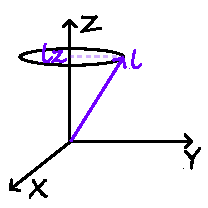
\includegraphics[width=0.8\linewidth]{image/lz.pdf}
    %\label{fig:}
\end{minipage}
\hfill
\begin{minipage}{0.45\textwidth}
    \begin{equation*}
    	\left\{
    	\begin{aligned}
    		&\hat{l}^2 Y(\theta, \varphi) = l(l+1) Y(\theta, \varphi)\\
    		&\hat{l}_z Y(\theta, \varphi) = m Y(\theta, \varphi)
    	\end{aligned}
    	\right.
    \end{equation*}
    \begin{equation*}
    	\vc{l} = \vc{l}_1 + \vc{l}_2 = \left\{
    	\begin{aligned}
    		l_1 &+ l_2\\
    		l_1 &+ l_2 -1\\
    		&\vdots\\
    		|l_1 &- l_2|
    	\end{aligned}
    	\right.
    \end{equation*}

\end{minipage}
	$    
    	l_z = m\hbar, \hspace{2 mm} m \in [-l, \ldots, 0, \ldots, l]
    $
    момент -- наибольшее значение проекции.

\begin{minipage}{0.45\textwidth}
    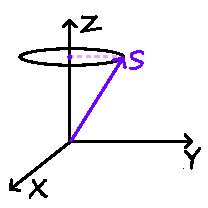
\includegraphics[width=0.8\linewidth]{image/s.pdf}
\end{minipage}
\hfill
\begin{minipage}{0.45\textwidth}
    \begin{equation*}
    	\left\{
    	\begin{aligned}
    		&\hat{s}^2 \chi(s) = s(s+1) \chi(s)\\
    		&\hat{s}_z \chi(s) = s_z \chi(s)
    	\end{aligned}
    	\right.
    \end{equation*}
    \begin{equation*}
    	\vc{s} = \vc{s}_1 + \vc{s}_2 = \left\{
    	\begin{aligned}
    		s_1 &+ s_2\\
    		s_1 &+ s_2 -1\\
    		&\vdots\\
    		|s_1 &- s_2|
    	\end{aligned}
    	\right.
    \end{equation*}
\end{minipage}
Отличие: момент $l$ --- только целый, спин $s$ -- целый и полуцелый.

Частицы с полуцелым спином называются фермионы. Примеры: электрон, протон, нейтрон, нейтрино спин $1/2$.

Частицы с целым спином --- бозоны. Примеры: пионы, спин 0, фотон -- спин 1 (условно).

Часто говорят, что спин -- это момент количества движения в системе покоя частицы. Это хорошо работает для массивных частиц, но требует уточнения для частиц с нулевой массой ($\gamma$-квант, нейтрино).

Но если спин не связан ни с каким реальным вращением в пространстве, то как же выглядит спиновая волновая функция и оператор спина?
Фактически у нас появилась некая дополнительная степень свободы: без учета спина у нас была фолновая функция $\psi(x,y,z,t)$.
А с учетом спина -- $\psi(x,y,z,t,\sigma)$, где $\sigma$ принимает два значение $+1/2$ и $-1/2$. Тогда имеет смысл ввести волновые функции $\psi_+(x,y,z,t)$ и $\psi_-(x,y,z,t)$ отличающиеся спиновой проекцией.
Это можно представить как
\begin{equation*}
	\psi(x,y,z,t,\sigma) = \psi(x,y,z,t)\chi_\sigma(s),
	\text{ где }
	\chi_{\frac{1}{2}}(s) = \left(\begin{aligned}1 \\ 0\end{aligned}\right),
	\text{ a }
	\chi_{-\frac{1}{2}}(s) = \left(\begin{aligned}0 \\ 1\end{aligned}\right).
\end{equation*}
Иногда обозначают спиновую часть волновой функции как 
\begin{equation*}
	\ket{\uparrow} = \left(\begin{aligned}1 \\ 0\end{aligned}\right),
	\hspace{5 mm}
	\ket{\downarrow} = \left(\begin{aligned}0 \\ 1\end{aligned}\right).
\end{equation*}
Комплексно сопряженная $\chi_{\frac{1}{2}}^*(s) = (1 \ 0)$.

Такая волновая функция называется спинором.
Мы привыкли, что скаляр -- это тензор нулевого ранга, вектор -- тензор первого ранга и так далее.
Спинор это, грубо говоря, тензор половинного ранга или как их "дразнят" полувекторами или недовекторами.
Это проявляется в том, что спинор ранга $1/2$ не переходит сам в себя при повороте на $360^\circ$, а только при повороте на $720^\circ$.

Как же выглядит оператор спина, переводящий столбец в другой?
Ясно, что это матрица $2 \times 2$.
Такие матрицы называются матрицами Паули
\begin{equation*}
	\hat{s}_x = \frac{1}{2} \hat{\sigma}_x = \frac{1}{2} \begin{pmatrix}
	    0 & 1 \\
	    1 & 0 \\
	\end{pmatrix},
	\hspace{2 mm}
	\hat{s}_y = \frac{1}{2} \begin{pmatrix}
	    0 & -i \\
	    i & 0 \\
	\end{pmatrix},
	\hspace{2 mm}
	\hat{s}_z = \frac{1}{2} \begin{pmatrix}
	    1 & 0 \\
	    0 & -1 \\
	\end{pmatrix}.
\end{equation*}

И ещё одна тонкость. В природе нет большим спинов отдельных частиц $s_\text{max} \leq 5/2$. Поэтому при $\hbar \to 0$, то $\hbar S \to 0$ и в классике спина нет!
Кроме того спин -- релятивистский объект, как было показано Дираком. При $1/c \to 0$ спин "исчезает".

Рассмотрим систему одинаковых частиц.
В классике мы можем "пометить" частицы и следить за их движениями по траекториям.
Но в квантовой физике траекторий нет и нет возможности "пометить" частицы. 
Таким образом все одинаковые частицы незримы -- так называемый признак тождественности частиц.

Пусть $1 \equiv (\vc{r}_1, \vc{s}_1)$ -- совокупность координат и спинов частицы 1. Аналогично $2 \equiv (\vc{r}_2, \vc{s}_2)$.
$\psi(1,2)$ -- волновая функция системы из двух частиц.
Переставим две частицы местами.
В силу тождественности $\psi(2,1) = k \psi(1,2)$, где $|k|^2 = 1$. 
Переставим ещё раз -- вернемся к исходной системе $\psi(1,2) = k \psi(2,1) = k^2 \psi(1,2)$ и $k^2 = 1$, $k = +1$ будет у бозонов, $k=-1$ будет у фермионов.

Обычно волновую функцию системы из двух частиц представляют в виде соответственно орбитальной и спиновой частей:
\begin{equation*}
	\psi(1,2) = \varphi(\vc{r}_1, \vc{r}_2) \chi_\sigma(\vc{s}_1, \vc{s}_2).
\end{equation*}
Переставляя частицы, мы переставляем из координаты и спины.
Для фермионов полня $\psi$-функция антисимметрична, следовательно, либо орбитальная симметрична относительно перестановки и спиновая антисимметрична, либо орбитальная антисимметрична, а спиновая симметрична.

Рассмотрим систему из двух электронов. Суммарный спин может ровняться или $1$ (3 проекции $+1$, $0$, $-1$) или $0$ (1 проекция $0$).
Попробуем построить соответствующие спиновые функции $\chi_\sigma(\vc{s}_1, \vc{s}_2)$ как произведение спиновых функций отдельных электронов.

При $S_z = +1$ означает, что $(s_1)_z = +1/2$ и $(s_2)_z = +1/2$, то есть $\chi_{+1}(s_1, s_2) = \ket{\uparrow}_1 \ket{\uparrow}_2$.

Аналогично, $S_z = -1$, означается, что $(s_1)_z = -1/2$ и $(s_2)_z = -1/2$, то есть $\chi_{+1}(s_1, s_2) = \ket{\downarrow}_1 \ket{\downarrow}_2$.

Что касается $S_z = 0$, то это соответствует либо $\chi_0(s_1,s_2) = \ket{\uparrow}_1 \ket{\downarrow}_2$, либо $\chi_0 (s_1, s_2) = \ket{\downarrow}_1, \ket{\uparrow}_2$.

Переставим местами электроны. Тогда
\begin{equation*}
	\chi_{+1} (s_2, s_1) = \begin{pmatrix}1 \\ 0\end{pmatrix}_2 \begin{pmatrix}1 \\ 0\end{pmatrix}_1 \equiv \begin{pmatrix}1 \\ 0\end{pmatrix}_1 \begin{pmatrix}1 \\ 0\end{pmatrix}_2
	=
	\chi_{+1}(s_1, s_2),
\end{equation*}
\begin{equation*}
	\chi_{-1} (s_2, s_1) = \begin{pmatrix}0 \\ 1\end{pmatrix}_2 \begin{pmatrix}0 \\ 1\end{pmatrix}_1 \equiv \begin{pmatrix}0 \\ 1\end{pmatrix}_1 \begin{pmatrix}0 \\ 1\end{pmatrix}_2
	=
	\chi_{-1}(s_1, s_2)
\end{equation*}
% все электроны тождественны.
\begin{equation*}
	\chi_0(s_2, s_1) = \begin{pmatrix}1 \\ 0\end{pmatrix}_2 \begin{pmatrix}0 \\ 1\end{pmatrix}_1
	\neq \chi_0(s_1, s_2),
\end{equation*}
\begin{equation*}
	\chi_0(s_2, s_1) = \begin{pmatrix}0 \\ 1\end{pmatrix}_2 \begin{pmatrix}1 \\ 0\end{pmatrix}_1
	\neq \chi_0(s_1, s_2).
\end{equation*}
Последние неравенство так же в наших обозначениях означают:
\begin{equation*}
	\ket{\uparrow}_2 \ket{\downarrow}_1 \neq \ket{\uparrow}_1 \ket{\downarrow}_2,
	\hspace{3 mm}
	\ket{\downarrow}_2 \ket{\uparrow}_1 \neq \ket{\downarrow}_1 \ket{\uparrow}_2.
\end{equation*}

Мы видим, что состояния с проекциями суммарного спина $\pm 1$ симметричны относительно перестановки, а состояния с проекциями $0$ не имеют никакой симметрии. Поскольку эта две возможности ($\ket{\uparrow}_1 \ket{\downarrow}_2$ и $\ket{\downarrow}_1 \ket{\uparrow}_2$) отвечают одной и той же суммарной проекции $0$, то мы не изменим это значения, если возьмём линейные комбинации $\frac{1}{\sqrt{2}}(\ket{\uparrow}_1 \ket{\downarrow}_2 \pm \ket{\downarrow}_1 \ket{\uparrow}_2)$ (множитель $\frac{1}{\sqrt{2}}$ введён для нормировки).

Но теперь комбинация со знаком "$+$" симметрична относительно перестановки $1 \to 2$, $2 \to 1$
\begin{equation*}
	\ket{\uparrow}_2 \ket{\downarrow}_1 + \ket{\downarrow}_1 \ket{\uparrow}_2 = \ket{\uparrow}_1 \ket{\downarrow}_2 + \ket{\downarrow}_2 \ket{\uparrow}_1.
\end{equation*}
Комбинация же со знаком "$-$" антисимметрична относительно перестановки $1 \to 2$, $2 \to 1$
\begin{equation*}
	\ket{\uparrow}_2 \ket{\downarrow}_1 - \ket{\downarrow}_2 \ket{\uparrow}_1 = -(\ket{\uparrow}_1 \ket{\downarrow}_2 - \ket{\downarrow}_1 \ket{\uparrow}_2).
\end{equation*}
Соответственно комбинация со знаком "$+$" соответствует проекции $0$ полного спина $1$, а со знаком "$-$" проекции $0$ полного спина $0$.
\begin{equation*}
	s=1\colon
	\left\{
	\begin{aligned}
		\chi_{+1} (s_1, s_2) =& \ket{\uparrow}_1 \ket{\uparrow}_2\\
		\chi_0 (s_1, s_2) =& \frac{1}{\sqrt{2}} (\ket{\uparrow}_1 \ket{\downarrow}_2 + \ket{\downarrow}_2 \ket{\uparrow}_1)\\
		\chi_{-1}(s_1, s_2) =& \ket{\downarrow}_1 \ket{\downarrow}_2
	\end{aligned}
	\right.
\end{equation*}
\begin{equation*}
	s = 0 \colon \left\{ \chi_0(s_1, s_2) = \frac{1}{\sqrt{2}} (\ket{\uparrow}_1 \ket{\downarrow}_2 - \ket{\downarrow}_1 \ket{\uparrow}_2)\right.
\end{equation*}

\textbf{Вывод}. При полном спине $1$ спиновая часть полной волновой функции  симметричная относительно перестановки, а при полном спине $0$ -- антисимметрична.

Значит при полном спине $1$ орбитальная волновая функция должна быть антисимметричной, а при полном спине $0$ -- симметричной.

Аналогично, если не учитывать взаимодействия (отталкивания) электронов, то орбитальная волновая функция двух электронов может быть представлена в виде произведения
\begin{equation*}
	\varphi(1,2) = \varphi_{n_1 l_1}(1) \psi_{n_2 l_2}(2),
\end{equation*}
где $\varphi_{n, l} (1)$ -- волновая функция (полная, то есть произведение радиальной на угловую части) 1-го электрона в состоянии с главным квантовым числом $n_1$ и орбитальным моментом $l_1$; $\psi_{n_2, l_2}(2)$ -- аналогично для второго электрона.
Однако $\varphi(1,2)$ не является ни симметричной, ни антисимметричной относительно перестановки электронов.
Так как эта функция и "переставленная" $\varphi(2,1)$ соответствует одной и той же суммарной энергии двух электронов, то из них можно построить две линейные комбинации
\begin{equation*}
	\frac{1}{\sqrt{2}}[\varphi_{n_1, l_1}(1) \psi_{n_2, l_2}(2) 
	\pm 
	\varphi_{n_1, l_1}(2) \psi_{n_2, l_2}(1)].
\end{equation*}
Теперь видно, что комбинация с "$+$" является симметричной относительно перестановки, а комбинация со знаком  "$-$" является антисимметричной.
Значит первая соответствует полному спину $0$, а вторая -- полному спину $1$.